\subsection{Response-aware differentiation without replacing the native world}
\label{sec:response-fidelity-v8}

Holding researcher weights fixed does not make their responses independent of
institutional inputs. We therefore retain the original forward world and learn
a local numeric response-boundary operator from native interventions, rather
than replacing the society by a smaller annual-state model. For institution
coordinates $\theta$, boundary replies $r$ and represented institutional loss
$S_T$, the differentiable representation composes
\[
 \frac{dS_T}{d\theta}=\partial_\theta S_T+
 \partial_r S_T\,\widehat J_r.
\]
The response Jacobian $\widehat J_r$ is fitted, not an exact LLM derivative.
The native review parser still applies its original integer conversion;
only the representation uses a declared soft staircase. Institution code,
tensor-to-tensor routing and recurrent memory remain in the composed backward
execution. Unknown record correspondence, changed contracts and controls
outside the calibration convex hull are unsupported, not zero gradients.

An explicit opt-in information-delivery capability connects actual institution
messages to actual review prompts, recording recipient, period, lineage and
prompt hashes. This closes a real ingress gap: the original review prompt does
not read generic institutional context. Default graphs retain identical prompt
bytes and scientific state. Generated institution source remains networkless
and sandboxed; this capability does not grant arbitrary host execution.

\paragraph{Scripted native implementation QA, not Qwen fidelity.}
Seven original six-year worlds use four original fixture researchers and
1,638 fresh \emph{scripted} replies. Within each year's review cohort the
scripted raw numeric score is uniform. This strict raw-parser adapter refuses
heterogeneous replies without a verified row correspondence; a general
post-parser boundary fit is separate, not silently treated as that adapter.
Three calibration controls
$[-.25,0,.25]$ give losses $[-72,-96,-96]$. Temperature .01 is selected using
only those calibration losses, before inspecting two predeclared unused
controls $[-.20,.10]$, whose losses are $[-72,-96]$.
Their finite difference is $-24$. A frozen-response predictor gives zero;
the response-aware autograd path integral gives $-23.99997638$, with absolute
error $2.36\times10^{-5}$. Both absolute endpoint checks also pass.
This is a finite-interval check of the scripted response rule, not a native
point Jacobian. The point gradient at zero is approximately $-3.21\times10^{-8}$.
A projected control .15999984 reevaluates to $-96$, tying rather than improving
the center. An extra control .6 yields native loss $-120$, but the representation
correctly declines prediction outside support; that outcome does not expand
support retrospectively.

\begin{figure}[t]
 \centering
 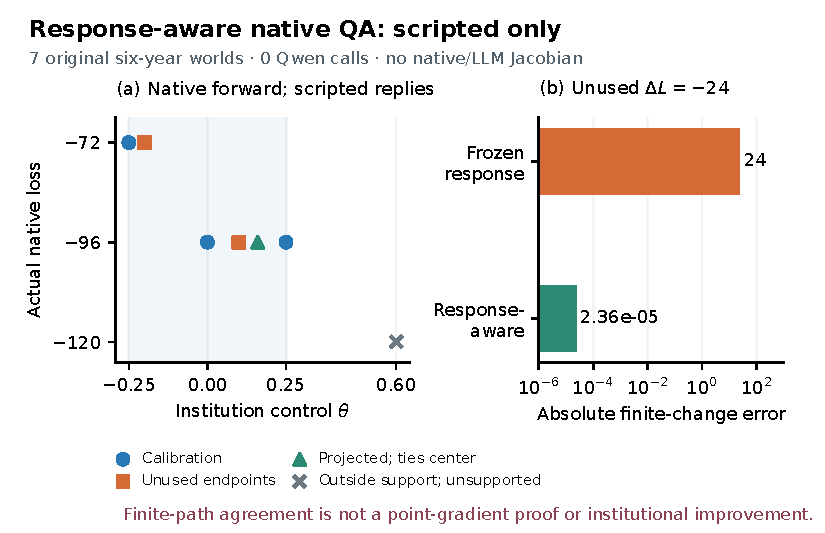
\includegraphics[width=\textwidth]{figures/native-response-fidelity-v8.pdf}
 \caption{Original-world response-boundary implementation QA with scripted
 replies, not empirical Qwen fidelity. Calibration, unused, proposed and
 unsupported native endpoints remain distinct. Finite-change agreement does
 not establish a useful point gradient or beneficial institutional design.}
 \label{fig:response-fidelity-v8}
\end{figure}

\paragraph{Failure and provenance boundaries.}
The first partial attempt fails because no actual review context reaches the
prompt; its temporary raw directory is subsequently lost, an explicit evidence
retention failure. A second batch completes five worlds before a scalar-type
handoff error; those raw worlds remain separately preserved. The successful
seven-world forward pin is \code{bfe83c0}. A separately pinned read-only analysis
hardens response attribution and refits the same endpoints without new forward
calls. Its 305-file raw inventory is unchanged. Three calibration response-file
hashes have historical saved-operator anchors; the other four endpoints have
full binding/count/task proof and posthoc checksums, not historical SQL seals.
A future completion-receipt API does not retroactively seal these runs.
Actual Qwen response fidelity, a whole-native pathwise derivative, and a
successful gradient-designed scientific institution remain unestablished.
